\chapter{Language Modeling: Foundations and Evolution}

In this chapter, I provide a comprehensive overview of language modeling, tracing its development from early statistical approaches to modern neural architectures. I begin by defining the language modeling task and explaining its fundamental principles. The discussion then progresses through key historical developments, including n-gram models, neural language models, and word embeddings, before examining contemporary large language models (LLMs) that have revolutionized natural language processing through their unprecedented scale and capabilities.

While the field has seen remarkable advances through scaling model size, there is growing recognition of the importance of efficient, smaller models that can operate in resource-constrained environments. This chapter therefore concludes with an exploration of recent innovations in training and deploying smaller language models, highlighting techniques that enable strong performance without the computational demands of their larger counterparts.

This foundation will set the stage for understanding the theoretical underpinnings and practical considerations of developing more efficient and accessible language models. 

\section{Language Modeling Task}
Language modeling refers to the task of assigning probabilities to sequences of words or tokens. The goal is to model the likelihood of a sequence in a language. In the case of a sequence of words, $w = w_1, w_2, \ldots, w_n$, the probability of the sequence is given by the product of the probabilities of the words occurring in the sequence:

\begin{equation}    
    P(w) = P(w_1, w_2, \ldots, w_n) = \prod_{i=1}^n P(w_i | w_1, \ldots, w_{i-1})
\end{equation}

Training a language model is then equivalent to estimating the parameters of this probability distribution. In practice, this is done by estimating the parameters of a neural network that maps a sequence of words to a probability distribution over the next word. 

\subsection{Early Approaches: N-Gram Models}
The earliest language models were based on n-gram statistics, where the probability of a word depends only on the preceding $n-1$ words. These models, described in foundational texts such as \cite{jurafsky2025speech}, are simple and effective but suffer from data sparsity and limited context. To address these issues, various smoothing techniques were developed, including Katz backoff \citep{katz2003estimation} and Kneser-Ney smoothing \citep{kneser1995improved}, with interpolated Kneser-Ney \citep{chen1999empirical} becoming the de facto standard for n-gram language modeling.

\subsection{Neural Language Models}

A major breakthrough came with the introduction of neural probabilistic language models by \cite{bengio2003neural}, which proposed using feed-forward neural networks to estimate the probability of word sequences. This approach introduced distributed word representations (embeddings), alleviating the data sparsity problem inherent in n-gram models. Subsequent work explored more powerful architectures, such as recurrent neural networks (RNNs) \citep{mikolov2010recurrent}, which can, in principle, capture dependencies across arbitrarily long contexts. However, training RNNs is challenging due to the vanishing and exploding gradient problems \citep{bengio1994learning}, leading to the development of gated architectures like Long Short-Term Memory (LSTM) networks \citep{hochreiter1997lstm} and Gated Recurrent Units (GRUs) \citep{cho2014gru}.
Large-scale empirical studies, such as \cite{jozefowicz2016exploring}, benchmarked various neural architectures and demonstrated that both model architecture and training data size significantly impact language modeling performance, as measured by perplexity.
\subsection{Word Embeddings}
In parallel, the adoption of distributed word representations, or word embeddings, marked a paradigm shift in NLP. Methods such as Skip-gram and Continuous Bag-of-Words (CBOW) \citep{mikolov2013efficient, mikolov2013distributed} and GloVe \citep{pennington2014glove} learn dense vector representations that capture syntactic and semantic relationships between words. These embeddings enabled transfer learning in NLP, as pre-trained vectors could be used for a variety of downstream tasks, including named entity recognition~\citep{lample2016neural}, sentence classification~\citep{kim2014convolutional}, and machine translation~\citep{qi2018translation}. However, traditional word embeddings are static, assigning the same vector to a word regardless of context.

Some novel methods have attempted to preproces or represent the input text data in unique ways, such as \cite{kim2016character} and phoneme-level representations \cite{goriely2024babble}.

\subsection{Contextualization and Attention}
To address the limitations of static embeddings, attention mechanisms were introduced, initially to solve the sequence alignment problem in machine translation \citep{bahdanau2015neural,luong2015effective}. Attention allows models to dynamically focus on relevant parts of the input sequence, improving translation quality and enabling the development of encoder-decoder architectures \citep{sutskever2014sequence}. The concept of contextual word embeddings was further advanced by models such as ELMo \citep{peters2018deep}, which extract context-sensitive representations from deep, bidirectional LSTMs.

\subsection{The Transformer and Modern Language Models}
The introduction of the Transformer architecture by Vaswani et al.~\citep{vaswani2017attention} marked a turning point in language modeling by replacing recurrence with self-attention mechanisms. This enabled efficient parallelization and the modeling of long-range dependencies, setting new performance benchmarks in machine translation and other NLP tasks. The Transformer built on earlier advances such as the soft attention mechanism of Bahdanau et al.~\citep{bahdanau2015neural}, which allowed neural machine translation models to dynamically align source and target sequences, improving translation quality and eliminating the need for a fixed-size encoding.

BERT~\citep{devlin2019bert} introduced the masked language modeling (MLM) objective, where some percentage of input tokens are replaced with a special [MASK] token, and the model is trained to predict the original identity of these masked tokens given their context. Formally, for a sequence of tokens $w = (w_1, \ldots, w_n)$ and a set of masked positions $M \subset \{1, \ldots, n\}$, the MLM objective maximizes
\begin{equation}
    \mathcal{L}_{\text{MLM}} = \sum_{i \in M} \log P(w_i \mid w_{\setminus M}),
\end{equation}
where $w_{\setminus M}$ denotes the sequence with masked tokens replaced by [MASK]. This enables BERT to learn deep bidirectional representations, as the model can attend to both left and right context. 

Following BERT, a number of variants improved on its design. RoBERTa~\citep{liu2019roberta} removed the next sentence prediction task and scaled up training data and compute. ALBERT~\citep{lan2019albert} introduced parameter sharing and sentence order prediction to reduce model size and improve efficiency. SpanBERT~\citep{joshi2020spanbert} focused on span-level objectives for better performance on related tasks. Other architectural innovations include DistilBERT~\citep{sanh2019distilbert}, which compresses BERT via knowledge distillation, and DeBERTa~\citep{he2021deberta}, which enhances attention mechanisms through disentangled representations.

In contrast to masked language modeling, autoregressive pretraining—as used in the GPT series~\citep{radford2018gpt1, radford2019gpt2, brown2020gpt3}—trains models to predict each token based only on its preceding context. This objective maximizes the likelihood:

\begin{equation}
\mathcal{L}_{\text{AR}} = \sum_{i=1}^n \log P(w_i \mid w_1, \ldots, w_{i-1}),
\end{equation}

enforcing a unidirectional, left-to-right dependency. Despite this constraint, autoregressive models have proven particularly effective for large-scale pretraining, and form the foundation of many state-of-the-art language models used today. Their simplicity and scalability have contributed to their widespread adoption for open-ended generation tasks.

Building on these two main paradigms, several models have explored alternative objectives and architectures. One especially influential direction is the encoder-decoder, or text-to-text, framework. T5~\citep{raffel2020t5} exemplifies this approach by casting all NLP tasks—classification, translation, question answering—as text generation problems within a unified pretraining scheme. Similarly, BART~\citep{lewis2020bart} combines a denoising autoencoder objective with a sequence-to-sequence architecture, enabling both robust understanding and fluent generation.

Other notable innovations include Transformer-XL~\citep{dai2019transformer}, which improves long-context modeling through segment-level recurrence and relative positional encodings; CTRL~\citep{keskar2019ctrl}, which allows controllable generation via conditioning on control codes; ELECTRA~\citep{clark2020electra}, which reframes pretraining as a discriminative task of replaced-token detection for improved sample efficiency; and XLNet~\citep{yang2019xlnet}, which generalizes autoregressive modeling using permutation-based objectives to capture bidirectional dependencies without masking.

Together, these advances reflect a broad exploration of architectures and training strategies, enabling the current generation of language models to achieve impressive results across a wide range of NLP tasks.

\subsection{Alternative Architectures}
While Transformers dominate large language modeling, recent research has explored alternative sequence modeling approaches to address their limitations, such as quadratic complexity and long-range dependency challenges. One promising direction is state space models (SSMs). The HiPPO framework~\citep{gu2020hippo} introduced efficient memory representations for continuous-time sequences, leading to the Structured State Space Sequence (S4) model~\citep{gu2021efficiently}, which models long-range dependencies efficiently via fast convolution. Mamba~\citep{gu2023mamba} further advances SSMs with dynamic, input-dependent state transitions, achieving Transformer-level performance with linear complexity. Another notable architecture, RWKV~\citep{peng2023rwkv}, combines features of Transformers and RNNs, replacing self-attention with a time-mixed mechanism for efficient, competitive language modeling. 

While these alternative architectures represent novel and important directions for efficient and expressive sequence modeling, in this thesis we focus primarily on Transformer-based models as the most successful and widely adopted approach for language modeling.

\subsection{Training and Optimization}

\paragraph{Optimization Algorithms.} The foundational method for training neural networks is stochastic gradient descent (SGD)\citep{robbins1951stochastic}, which iteratively updates model parameters using noisy gradient estimates from mini-batches. To address limitations in learning rate tuning and convergence speed, a range of adaptive optimizers have been developed. These include Adagrad\citep{duchi2011adaptive}, which adapts learning rates based on historical gradients; RMSProp~\citep{tieleman2012lecture}, which normalizes updates using a moving average of squared gradients; Adam~\citep{kingma2015adam}, which combines momentum with adaptive learning rates; and AdamW~\citep{loshchilov2019decoupled}, which decouples weight decay from the gradient update, improving regularization behavior.
In practice, effective training of deep networks also relies on learning rate scheduling and gradient clipping. For example, the Transformer architecture~\citep{vaswani2017attention} employs a learning rate schedule with an initial warm-up phase followed by inverse square root decay. Additionally, gradient clipping~\citep{pascanu2013difficulty}—scaling gradients when they exceed a threshold—is essential for preventing exploding gradients, a technique that has proven crucial for training recurrent neural networks and stabilizing large-scale Transformer models.

\paragraph{Activation Functions.} 

An activation function is a mathematical operation applied to each neuron's output in a neural network, introducing nonlinearity and enabling the network to learn complex patterns. Activation functions are central to the expressiveness and trainability of neural networks. Early neural networks, as in the foundational work on backpropagation~\citep{rumelhart1986learning}, primarily used the sigmoid activation. \citet{lecun1998efficient} analyzed practical choices for activations, showing that $\tanh$ is preferable to sigmoid due to its zero-centered output, which improves optimization dynamics.

However, both sigmoid and $\tanh$ suffer from vanishing gradients in deep networks, as highlighted by \citet{glorot2010understanding}. This limitation motivated the adoption of the Rectified Linear Unit (ReLU)~\citep{nair2010rectified}, defined as $\mathrm{ReLU}(x) = \max(0, x)$, which is computationally simple and alleviates vanishing gradients. ReLU became the default activation in deep learning throughout the 2010s and is still used in some lightweight transformer variants. Variants such as Leaky ReLU~\citep{maas2013rectifier} allow a small gradient for negative inputs, helping to prevent the ``dying ReLU'' problem, and have seen use in audio and speech models.

For modern language models, smoother and non-monotonic activations have proven more effective. The Gaussian Error Linear Unit (GELU)~\citep{hendrycks2016gaussian} became the default in BERT and subsequent transformers due to its empirical gains over ReLU. Swish~\citep{ramachandran2017searching}, defined as $\mathrm{Swish}(x) = x \cdot \mathrm{sigmoid}(\beta x)$, is another smooth, non-monotonic activation that performs well in deep and convolutional models. More recently, gated activations such as SwiGLU~\citep{shazeer2020glu}—which combines Swish and linear units—have outperformed ReLU and earlier GLU variants in transformer feedforward networks.

The evolution of activation functions reflects the ongoing search for improved expressiveness, optimization, and stability in deep neural architectures.

\paragraph{Regularization and Stabilization.} Overfitting occurs when a model learns not only the underlying patterns in the training data but also the noise, resulting in poor generalization to new, unseen data. To address this, regularization techniques such as dropout~\citep{srivastava2014dropout} are employed, which randomly deactivate units during training to encourage robustness and prevent reliance on specific features.

In addition to regularization, normalization methods play a crucial role in stabilizing training and further improving generalization. \textbf{Batch Normalization}~\citep{ioffe2015batchnorm} normalizes activations over a mini-batch, but is less common in language models due to variable sequence lengths. Instead, \textbf{Layer Normalization}~\citep{ba2016layernorm} is widely used in RNNs and Transformers, as it normalizes across features within each data point, improving stability regardless of batch size. \textbf{RMSNorm}~\citep{zhang2019rmsnorm}, a simplified variant omitting mean subtraction, is used in models like T5 and GPT-J. The placement of normalization layers has evolved: the original Transformer~\citep{vaswani2017attention} used \emph{Post-LN} (after residuals), but this can destabilize deep models. \emph{Pre-LN}~\citep{xiong2020layer}, where normalization is applied before each sublayer, is now standard in most modern LMs for improved stability.

\paragraph{Architectural Enhancements.}
A crucial architectural component in Transformer-based models is the method for encoding token position, which allows models to incorporate sequence order into otherwise permutation-invariant self-attention mechanisms. The original Transformer~\citep{vaswani2017attention} introduced \emph{sinusoidal positional encodings}, which are added to token embeddings and provide a fixed, non-learned way to represent absolute position. In contrast, models such as GPT~\citep{radford2018gpt1} and BERT~\citep{devlin2019bert} use \emph{learned positional embeddings}, which offer greater flexibility but may generalize poorly to longer contexts unless specifically augmented.

To address the limitations of absolute position encodings, \citet{shaw2018self} proposed \emph{relative position representations}, allowing the model to encode the distance between tokens directly in the attention mechanism. This approach is particularly important for enabling models to generalize to longer contexts and to be less dependent on a fixed sequence length. Further innovations include \emph{linear attention biases} (ALiBi)~\citep{press2021train}, which add a simple, non-learned bias to the attention scores based on token distance. Another widely adopted method is the \emph{Rotary Position Embedding} (RoPE)~\citep{su2024rope}, which applies rotary transformations to the key and query vectors in the attention mechanism. RoPE has become popular in many large models, such as LLaMA, due to its strong extrapolation capabilities and implementation simplicity.

Beyond positional encoding, several other architectural enhancements have become standard in modern Transformers. \emph{Residual connections}~\citep{he2016deep}, originally introduced in ResNets to address vanishing gradients, are essential for enabling the training of deep Transformer models by facilitating gradient flow. More recent innovations include \emph{Grouped Query Attention} (GQA)~\citep{ainslie2023gqa}, which reduces memory and compute requirements by grouping multiple attention heads to share key and value projections—a technique now adopted in models such as Gemini, PaLM, and LLaMA. Additionally, parameter efficiency has been improved through \emph{weight tying}~\citep{press2017using}, where the input and output embedding matrices are shared, reducing the number of parameters without sacrificing performance

\subsection{Scaling and Architecture Search}
While recent research has shown that scaling model and dataset size leads to predictable improvements in performance~\citep{kaplan2020scaling, henighan2020scaling}, designing neural network architectures in a robust and rigorous way remains a significant challenge. Much of architecture design is still guided by empirical intuition and trial-and-error, rather than first principles. For example, \citet{levine2020depth} offer a structured perspective on the trade-offs between scaling depth and width in Transformers, proposing guidelines for balancing these factors under a fixed compute budget. The scaling laws established by \citet{kaplan2020scaling} demonstrate that both wider and deeper models can improve performance if scaled appropriately, but do not prescribe how to select specific architectural configurations for a given task or resource constraint.

To address the difficulty of manual architecture design, neural architecture search (NAS) methods have been developed to automate this process. Early work by \citet{zoph2017neural} introduced the use of reinforcement learning to train a controller network that proposes architectures, using the accuracy of candidate models as a reward signal. More recent approaches have applied NAS specifically to Transformer models: AutoFormer~\citep{chen2021autoformer} efficiently searches over large design spaces (such as number of heads, depth, and MLP size) using weight-sharing, while NAS-BERT~\citep{xu2021nasbert} tailors BERT-like architectures for specific NLP tasks, reducing model size while maintaining performance through task-conditioned optimization.

Despite these advances, finding good architectures remains challenging and is difficult to do rigorously. Automated methods like NAS are increasingly important for discovering efficient and effective models, but robust principles for architecture design are still an open research area.


\section{Large Language Models}

The advent of large language models (LLMs) marked a turning point in natural language processing. Unlike earlier models, which were limited by data and compute, LLMs are trained on massive corpora and contain billions or even trillions of parameters. This scale enables them to perform a wide range of tasks—including question answering, summarization, translation, and code generation—often with little or no task-specific training. It is important to note, however, that the definition of ``large'' in large language models is a moving target: as models and hardware have advanced, what was once considered large has quickly become standard or even small by contemporary benchmarks.

The rapid progress in large language models has been marked by influential systems, each pushing the boundaries of scale, capability, and accessibility. GPT-3~\citep{brown2020gpt3} established the transformative potential of large transformer-based models, enabling tasks in few-shot or zero-shot settings. GPT-4~\citep{openai2023gpt4} further expanded scale and capabilities, emphasizing the complexities of evaluating massive models.

Open-source models have also significantly advanced the field. DeepSeek LLM~\citep{deepseek2024llm} optimizes hyperparameters aligned with scaling laws, while Mistral 7B~\citep{jiang2023mistral} introduces efficiency-driven architectural innovations. Similarly, PaLM~\citep{chowdhery2023palm}, OPT~\citep{zhang2022opt}, and BLOOM~\citep{le2023bloom} contribute distinct approaches to scaling and transparency, with LLaMA models~\citep{touvron2023llama} emphasizing research optimization.

Furthermore, models like Anthropic's Claude~\citep{anthropic2024claude3,anthropic2024claude35,anthropic2025claude37}, Google's Gemini~\citep{deepmind2023gemini}, Baidu's ERNIE 4.0~\citep{baidu2023ernie4}, and Alibaba's Qwen~\citep{alibaba2023qwen} demonstrate advancements in multimodality, language specificity, and principled AI, showcasing diverse avenues of progress in large-scale language modeling.

The following section explores some of the critical aspects of large language models including their pre-training datasets, large-scle evaluation benchmarks, and properties.

\subsection{Datasets for Large Language Model Pretraining}
The performance of large language models (LLMs) is strongly influenced by the scale, diversity, and quality of their pretraining datasets. Over the past several years, a number of large-scale corpora have been developed to support open and reproducible LLM research. Table~\ref{tab:llm-datasets} summarizes some of the most widely used datasets.
\begin{table}[h]
\centering
\begin{tabular}{p{3.5cm} p{1.5cm} p{8.5cm}}
\toprule
\textbf{Dataset} & \textbf{Size} & \textbf{Type of Data} \\
\midrule
OpenWebText~\citep{gokaslan2019openweb} & $\sim$8B & Web, Wikipedia \\
BooksCorpus~\citep{zhu2015aligning} & $\sim$0.8B & Fiction books \\
The Pile~\citep{gao2020pile} & 250B & Web, academic, code, books, forums \\
C4~\citep{raffel2020t5} & 365B & Web (Common Crawl) \\
RedPajama~\citep{together2023redpajama} & 1.2T & Web, books, Wikipedia, code, academic \\
RefinedWeb~\citep{penedo2023refinedweb} & 600B & Web (Common Crawl) \\
FineWeb~\citep{penedo2024fineweb} & 15T & Web, education \\
DOLMa~\citep{soldaini2024dolma} & 3T & Web, Wikipedia, books, code, academic, forums \\
\bottomrule
\end{tabular}
\caption{Major datasets used for large language model pretraining, with approximate number of tokens and data types.}
\label{tab:llm-datasets}
\end{table}
These datasets are constructed from a variety of sources, including web pages (Common Crawl), books, academic papers, code repositories, and community forums. Notably, OpenWebText~\citep{gokaslan2019openweb} and BooksCorpus~\citep{zhu2015aligning} were foundational for early models like GPT-2 and BERT, while The Pile~\citep{gao2020pile} and C4~\citep{raffel2020t5} introduced greater diversity and scale. More recent efforts such as RedPajama~\citep{together2023redpajama}, RefinedWeb~\citep{penedo2023refinedweb}, FineWeb~\citep{penedo2024fineweb}, and DOLMa~\citep{soldaini2024dolma} focus on openness, quality filtering, and massive scale, supporting the next generation of open LLMs.

\subsection{Evaluation Benchmarks for Large Language Models}
The advancemnet of large language models (LLMs) has also been driven by the development of rigorous evaluation benchmarks. These benchmarks assess a model's ability to understand, reason, and generate language across a wide range of tasks. Below, we summarize some of the most influential benchmarks used to evaluate LLMs.
\paragraph{GLUE and SuperGLUE.} The General Language Understanding Evaluation (GLUE) benchmark \citep{wang2018glue} popularized the paradigm of transfer learning and fine-tuning in NLP. It consists of nine tasks, including natural language inference (MNLI, RTE) \citep{williams2018mnli,dagan2006rte}, paraphrase detection (MRPC) \citep{dolan2005mrpc}, sentiment analysis (SST-2) \citep{socher2013sst}, linguistic acceptability (CoLA) \citep{warstadt2019cola} and semantic similarity (STS-B) \citep{cer2017stsb}. BERT's breakthrough performance on GLUE established it as a standard benchmark, but as models approached the performance ceiling, overfitting became a concern. SuperGLUE \citep{wang2019superglue} was introduced as a more challenging successor, featuring tasks that require multi-sentence reasoning, commonsense inference, and coreference resolution \citep{zhang2018record,pilehvar2019wic,khashabi2018multirc,roemmele2011copa}. Progress on these benchmarks has closely tracked advances in LLM capabilities.

\paragraph{MMLU.} The Massive Multitask Language Understanding (MMLU) benchmark \citep{hendrycks2021mmlu} evaluates models on 57 diverse tasks spanning STEM, humanities, law, and more, using multiple-choice questions. MMLU emphasizes zero-shot and few-shot generalization, and is now a standard for evaluating the broad knowledge and reasoning abilities of frontier LLMs such as GPT-3, GPT-4, Claude, and LLaMA.

\paragraph{ARC.} The AI2 Reasoning Challenge (ARC) \citep{clark2018arc} tests scientific and commonsense reasoning using grade-school multiple-choice questions. The challenge set is specifically designed to be unsolvable by information retrieval alone, requiring genuine reasoning and world knowledge.

\paragraph{BIG-Bench and BIG-Bench Hard.} The Beyond the Imitation Game Benchmark (BIG-Bench) \citep{suzgun2023bigbenchhard} is a large-scale suite of over 200 tasks covering math, code, ethics, linguistics, and more, designed to probe

\paragraph{HellaSwag.} HellaSwag: Can a Machine Really Finish Your Sentence?~\citep{zellers2019hellaswag} is a commonsense inference benchmark that evaluates a model's ability to complete sentences in a grounded and contextually appropriate manner. Each example presents a context followed by four possible sentence endings, and the model must select the most plausible continuation. HellaSwag is specifically designed to be challenging for language models by minimizing the effectiveness of superficial statistical cues, thereby requiring genuine understanding of everyday scenarios and commonsense reasoning. This benchmark is widely used to assess whether models can move beyond surface-level pattern matching to deeper contextual comprehension.

\paragraph{Intrinsic Evaluation: Perplexity and Linguistic Probes.} Perplexity \citep{jelinek1977perplexity} remains a standard metric for evaluating the predictive quality of language models, though it does not capture all aspects of language understanding. Recent work \citep{magnusson2024paloma} argues for broader evaluation frameworks, including statistical properties of generated text. Linguistic benchmarks such as BLiMP \citep{warstadt2020blimp} and MSGS \citep{warstadt2020msgs} probe syntactic, semantic, and morphological competence, while Paloma \citep{magnusson2024paloma} measures how well models fit real-world human text distributions.
These benchmarks collectively provide a comprehensive picture of LLM capabilities, from basic language understanding and reasoning to factuality, safety, and linguistic competence. As models continue to improve, the development of new and more challenging benchmarks remains essential for tracking progress and diagnosing limitations.

\subsection{Properties of Large Language Models}

Large language models (LLMs) exhibit a range of remarkable properties that set them apart from earlier generations of language models. As these models have grown in scale and sophistication, researchers have observed the emergence of new abilities, improved generalization, and the development of empirical scaling laws that guide model design. In addition, a suite of post-training methods has been developed to further enhance LLM capabilities, aligning them more closely with human preferences and real-world requirements.

\paragraph{Emergent Abilities}

A striking phenomenon in LLMs is the appearance of emergent abilities—capabilities that arise unpredictably as model size increases. For example, certain tasks such as arithmetic reasoning and multi-step problem-solving are only performed successfully by models beyond a specific scale \citep{{wei2022emergent}}. Some studies reveal that performance on particular tasks follows U-shaped or inverted-U scaling curves, allowing for the prediction of emergence thresholds and future performance \citep{wu2024u}. However, this unpredictability has been challenged, with some arguing that emergent abilities may be artifacts of how performance is measured, and that with appropriate evaluation, their appearance can be anticipated \citep{schaeffer2023mirage}. Notably, reasoning abilities such as chain-of-thought prompting emerge naturally in sufficiently large models, enabling them to solve complex problems by generating intermediate reasoning steps \citep{wei2022chain}


\paragraph{Generalization}

Closely related to emergence is the property of generalization. LLMs are able to perform well on unseen data, often surpassing expectations for overparameterized models \citep{belkin2019reconciling}. Research has shown that increasing model capacity beyond the point of interpolation can actually improve test performance, depending on the task. Many few-shot prompting abilities only emerge around 100-500B parameters, and over 1E+23 flops roughly. This is demonstrated empirically on linear models, neural networks, and kernel methods. \citet{yilmaz2022regularization} provide a theoretical exploration of why deep double descent occurs, relating to interpolation threshold, noise, and regularization, and providing insights for how and when overparameterized models avoid overfitting.


\paragraph{Scaling Laws}

The development and scaling of LLMs have been guided by empirical scaling laws, which describe how model performance depends on factors such as model size, dataset size, and compute. \citet{kaplan2020scaling} establish a power-law relationship between these factors, recommending making models bigger while keeping the training dataset size relatively fixed. \citet{henighan2020scaling} extend these laws to a multimodal setting, showing that larger models continue improving even on out-of-distribution data. \citet{hoffman2022chinchilla} introduce the Chinchilla model, finding that models trained with more data for longer, but with fewer parameters, perform better for the same amount of compute, suggesting that data size should scale more aggressively than model size to be compute-optimal. \citet{hernandez2021scaling} explore how scaling affects transfer performance to downstream tasks, finding that larger models require less fine-tuning data, and downstream task performance also follows predictable scaling curves.

\subsection{Post-Training Methods for Large Language Models}

Beyond pretraining, recent advances in LLMs have been driven by sophisticated post-training methods that enhance factuality, alignment, and task performance. One prominent direction is retrieval-augmented generation (RAG), which adds non-parametric memory to language models~\citep{lewis2020retrieval}. This approach enables LLMs to access up-to-date and domain-specific information beyond their training data, achieving state-of-the-art results on knowledge-intensive tasks. Some models, such as Command R+~\citep{cohere2024commandrplus}, are fine-tuned specifically for retrieval-augmented workflows and to improve their factual accuracy.

Another major area of post-training is alignment with human preferences and instructions. Reinforcement learning from human feedback (RLHF)~\citep{christiano2017deep, ouyang2022training} with Proximal Policy Optimization (PPO)~\citep{schulman2017proximal} has become a standard method to fine-tune models using reward signals from human preference data. Direct Preference Optimization (DPO)~\citep{rafailov2023direct} is an alternative approach that directly optimizes model parameters from preference data, bypassing the need for a separate reinforcement learning loop. This method is used in recent open-source models such as Zephyr~\citep{huggingface2023zephyr}, which are chat-tuned for high-quality conversational performance. Instruction finetuning is another effective post-training strategy. Models like InstructGPT~\citep{ouyang2022training} and FLAN~\citep{wei2021flan} are further trained on instruction datasets, often with human feedback, that greatly improving their ability to follow instructions, and generate helpful outputs. Within instruction finetuning, including chain-of-thought reasoning in the finetuning data has been shown to further boost performance on complex tasks \citep{wei2022chain}.

Collectively, these post-training methods are critical for aligning LLMs with human values, improving factuality, and enabling robust performance across a wide range of real-world applications.

\section{Small Language Models}

The landscape of language modeling has rapidly expanded beyond massive models like GPT-3 and GPT-4, giving rise to a vibrant ecosystem of smaller language model frameworks. Several open-source projects, such as the OPT language model family~\citep{zhang2022opt}, Pythia \citep{biderman2023pythia} and OLMo \citep{groeneveld2024olmo}, have played a key role in democratizing access to large-scale language modeling by releasing models of varying sizes (including sub-1 biliion parameter models) and making their implementations widely available. Other initiatives, such as LaMini-LM~\citep{wu2024lamini} and TinyLlama~\citep{zhang2024tinyllama}, have focused on developing tiny-scale, instruction-tuned models similar to ChatGPT that are capable of following instructions and solving language understanding tasks.

In parallel, the demand for on-device deployment and cost-effective inference has spurred the development of numerous small language model suites. Frameworks such as MobileLLM~\citep{liu2024mobilellm} and Microsoft's Phi-3~\citep{abdin2024phi} are specifically optimized for mobile and resource-constrained environments, addressing challenges related to latency, memory, and efficiency. Other projects, including Apple's OpenELM~\citep{mehta2024openelm} and MobiLlama~\citep{thawakar2024mobillama}, focus on minimizing battery consumption through energy-efficient model architectures.

Together, these frameworks reflect the growing demand for practical and versatile NLP tools that can operate in diverse environments. In the following section, we will examine a broad set of existing strategies to make small language models more efficient to train and deploy.

\subsection{Hyper-Parameter Selection}

Recent work has shown that simply carefully tuning hyper-parameter selection can dramatically improve the efficiency and performance of small language models, even under tight computational constraints. Approaches such as targeted architectural choices~\citep{hillier2024super}, optimized training schedules and mixed-precision techniques~\citep{izsak2021train}, and aggressive learning rate strategies~\citep{geiping2023cramming} enable strong results on standard benchmarks using limited resources.

\subsection{Software Packages}

A number of specialized software frameworks have been developed to enable efficient training of large language models on modern hardware. Megatron-LM~\citep{narayanan2021megatron} and DeepSpeed~\citep{rasley2020deepspeed} introduce advanced parallelism strategies and memory optimizations, such as tensor and pipeline model parallelism, ZeRO redundancy optimizer, and 3D parallelism, allowing models to be trained efficiently across GPU clusters. These tools emphasize scalability, throughput, and hardware efficiency, making language modeling pre-training feasible with limited resources~\citep{rajbhandari2020zero}.


\subsection{Knowledge Distillation}

Knowledge distillation is a central technique for training small language models, particularly in data-limited settings. Here, a compact student model learns to replicate the behavior of a larger teacher or an ensemble, often improving efficiency and performance.
Recent studies show that distillation can be highly effective even when both teacher and student are small. For example, \citet{timiryasov2023baby} and \citet{tastet2024babyllama2} demonstrate that distilled models can outperform their teachers and baselines on the BabyLM benchmark, highlighting the value of ensemble and distillation strategies when data is scarce. \citet{yam2024tinyminds} further show that careful distillation design can yield gains even with compact models, improving on strong baselines like LTG-BERT.
Distillation is also used in widely adopted models such as DistilBERT~\citep{sanh2019distilbert}, which achieves a smaller, faster, and more efficient version of BERT with minimal accuracy loss. Beyond efficiency, distillation can enhance advanced capabilities: for instance, Deepseek-r1~\citep{guo2025deepseekr1} leverages distillation from a larger Qwen model to improve reasoning abilities in the student.

\subsection{Pruning}

Unlike knowledge distillation, which transfers knowledge from a larger teacher to a smaller student model, pruning directly reduces model size by removing unnecessary weights or connections from a trained network. This approach aims to create sparse, efficient models without requiring a separate teacher.
Early work such as Optimal Brain Damage~\citep{lecun1990optimal} and Optimal Brain Surgeon~\citep{hassibi1993optimal} introduced principled pruning based on second-order derivatives of the loss, identifying and removing weights with minimal impact on performance. Later, magnitude-based pruning~\citep{han2015learning} offered a scalable alternative by eliminating low-magnitude weights, followed by retraining to recover accuracy. This method was extended in Deep Compression~\citep{han2016deep}, which combines pruning, quantization, and coding to dramatically reduce model size for deployment on devices like smartphones.
The Lottery Ticket Hypothesis~\citep{frankle2019lottery} further showed that large, dense networks contain sparse subnetworks (“winning tickets”) that can be trained to match the original model's accuracy, suggesting that much of a model's capacity is redundant. More recently, efficient single-shot pruning methods such as Wanda~\citep{sun2024simple} have been proposed, using weight magnitude and input activation norms to identify important weights without iterative retraining.
Pruning thus provides a complementary path to model efficiency, enabling substantial reductions in size and compute while maintaining strong performance.

\subsection{Architecture}

Modifications to the architecture of language models remains one of, if not the, most common approach for improving the efficiency of language models. In this section, we outline key approaches that have been proposed to reduce parameter count, memory usage, and computational cost.

\paragraph{Weight Decomposition}
A number of recent models exemplify these architectural innovations. LTG-BERT~\citep{samuel2023ltgbert}, for instance, integrates GEGLU activations with disentangled attention to separately encode content and positional information within the attention mechanism, thereby enhancing representational power without increasing model size. MobiLlama~\citep{thawakar2024mobillama} is designed for lightweight deployment and employs grouped query attention and shares weights between feed-forward layers to reduce redundancy and memory footprint. Similarly, MobileLLM~\citep{liu2024mobilellm} targets on-device applications by addressing latency and cost constraints through deep, thin architectures that utilize embedding sharing and block-wise grouped query attention for efficient inference. ALBERT~\citep{lan2019albert} further demonstrates the benefits of parameter sharing by tying the weights of both feed-forward and attention layers across the network, significantly reducing model size while maintaining strong performance.

\paragraph{Mixture-of-Experts and Conditional Computation}
Another major direction for architectural efficiency is the use of Mixture-of-Experts (MoE) and conditional computation, where only a subset of model parameters are activated for each input. The foundational idea was introduced by \citet{jacobs1991adaptive}, who proposed a gating mechanism to dynamically route information to different expert subnetworks, allowing the model to specialize and improve efficiency. Building on this, \citet{shazeer2017outrageously} demonstrated the effectiveness of sparsely-gated MoE layers in large-scale neural networks, applying conditional computation to language modeling and machine translation, initially with LSTM-based architectures. The approach was further advanced by Switch Transformers~\citep{fedus2021switch}, which implemented MoE within the Transformer framework for the first time, achieving up to a 7x increase in pre-training speed on T5-based models by activating only a subset of experts per input. More recently, Mixtral of Experts~\citep{jiang2024mixtral} introduced a sparse MoE architecture based on Mistral 7B, where each feedforward block selects from eight distinct expert groups, and a router network chooses two experts per token at each layer, enabling efficient scaling with minimal loss in performance.  GShard~\citep{lepikhin2020gshard} further contributed by introducing automatic sharding techniques for MoE architectures, facilitating the training of giant models across distributed hardware. The Deepseek-v3 model~\citep{deepseek2024v3} combines MoE with multi-head latent attention, exemplifying the latest advances in leveraging expert specialization and conditional computation for both scalability and efficiency in modern language models.


\paragraph{Sparse and Efficient Attention Mechanisms}
A central challenge in scaling language models is the quadratic computational and memory cost of standard self-attention, which motivates a wide range of approaches for making attention more efficient and scalable. Early work such as \citet{luong2015effective} introduced local attention for neural machine translation, restricting the attention mechanism to a fixed window around each token and thereby reducing computation by focusing only on relevant parts of the input. Building on this, a series of sparse attention mechanisms have been proposed to further improve efficiency for long sequences. The Sparse Transformer~\citep{child2019generating} utilizes a combination of strided and fixed attention patterns across layers, reducing complexity from $O(n^2)$ to $O(n\sqrt{n})$. The Routing Transformer~\citep{roy2020efficient} employs content-based sparse attention by dynamically clustering tokens using online k-means, achieving $O(n^{1.5})$. complexity. Longformer~\citep{beltagy2020longformer} and BigBird~\citep{zaheer2020big} combine local windowed attention with global and random attention patterns, enabling linear scaling with sequence length while maintaining strong empirical and theoretical performance. Reformer~\citep{kitaev2020reformer} introduces locality-sensitive hashing to group similar tokens into buckets, performing attention only within buckets and reducing complexity to $O(n\log(n))$; it also introduces reversible layers to minimize memory usage during training. Linformer~\citep{wang2020linformer} projects key and value matrices to a lower dimension, leveraging the low-rank property of attention matrices to achieve linear complexity. LongNet~\citep{ding2023longnet} proposes a hierarchical, dilated attention pattern that, when combined with stacked layers, allows models to attend to a wide range of tokens efficiently, scaling to extremely long sequences. More recent innovations include attention sinks~\citep{xiao2023attentionsink}, which introduce special tokens that accumulate attention and serve as memory anchors, improving streaming model performance.
In addition to algorithmic sparsity, hardware-aware optimizations have also played a crucial role. FlashAttention~\citep{dao2022flashattention} and its successor FlashAttention-2~\citep{dao2023flashattention2} achieve dramatic speed and memory improvements by tiling the attention computation to fit on-chip memory, minimizing slow memory accesses and fusing operations into a single GPU kernel. These methods compute exact softmax attention (unlike many sparse or approximate methods), enabling models to process much longer sequences—up to 16K tokens or more—without sacrificing accuracy or requiring architectural changes. FlashAttention-2 further improves efficiency by supporting variable-length sequences and mixed precision, achieving up to 3x speedups and better GPU utilization. Collectively, these advances in sparse and efficient attention mechanisms have been instrumental in enabling the training and deployment of large language models on long-context tasks and resource-constrained hardware.

\paragraph{Adapters and Parameter-Efficient Fine-Tuning}

For fine-tuning large pre-trained models on downstream tasks, adapters and parameter-efficient fine-tuning (PEFT) methods have become essential. Instead of updating all model parameters, these approaches introduce small trainable modules or selectively update a subset of parameters, greatly reducing computational and memory costs. Early work in vision~\citep{rebuffi2017adapters} added residual adapter modules, while in NLP, \citet{houlsby2019parameter} proposed lightweight down- and up-projection layers within Transformers. LoRA~\citep{hu2021lora} further improved efficiency by injecting low-rank trainable matrices into attention and feed-forward layers, enabling adaptation with minimal parameters and no added inference latency. ReLoRA~\citep{lialin2023relora} extends this by using low-rank updates for faster, more memory-efficient training. Other PEFT strategies include BitFit~\citep{benzaken2022bitfit}, which updates only bias terms, and (IA)$^3$~\citep{liu2022few}, which scales activations with learned vectors for even greater parameter savings. Tools like HuggingFace's PEFT library have made these techniques widely accessible, enabling rapid and cost-effective adaptation of large models to new tasks.

\subsection{Quantization}
Quantization reduces the memory and compute demands of large language models by representing weights and activations with low-precision values. BitNet~\citep{wang2023bitnet} achieves extreme efficiency by binarizing weights to a single bit and scaling activations with an absmax function, while keeping gradients in full precision. Activation-Aware Weight Quantization~\citep{lin2023awq} preserves accuracy by expanding the range of the most important weights, minimizing distortion from low-bit quantization. QLoRA~\citep{dettmers2023qlora} enables efficient fine-tuning of 4-bit quantized models by adding a small set of trainable low-rank weights, making it possible to adapt large models like LLaMA-65B on a single GPU. Underpinning many quantization methods is the Straight-Through Estimator (STE)~\citep{bengio2013estimating}, which allows gradients to flow through non-differentiable quantization operations. Together, these advances make it feasible to compress and deploy large models in resource-limited settings.


\subsection{Data Calibration}

Recent research has demonstrated that carefully calibrated training data can enable small language models to achieve surprisingly strong performance, challenging the conventional wisdom that massive datasets are always necessary. This insight has important implications for developing more efficient and accessible language models.

One notable example is the TinyStories dataset~\citep{eldan2023tinystories}, which consists of approximately 1.3 million synthetic short children's stories generated by GPT-3.5 and GPT-4. By using a limited vocabulary of around 1,500 words and focusing on simple, coherent narratives, TinyStories enables small models to learn effective language generation without requiring massive amounts of data. This approach demonstrates that controlled, high-quality training data can be more valuable than raw data quantity.

Similarly, BabyBERTa~\citep{huebner2021babyberta} shows that specialized datasets of child-directed speech can help small models acquire sophisticated grammatical knowledge. By training on just 5 million words of language targeted at 1-6 year olds, BabyBERTa achieves grammatical capabilities comparable to larger models while using 15 times fewer parameters and 6,000 times less training data. This suggests that the quality and nature of training data can significantly impact model efficiency.

The relationship between data scale and model capabilities was further explored by \citet{zhang2021need}, who identified distinct thresholds for different types of linguistic knowledge. Their work shows that models can effectively learn syntactic and semantic features with relatively modest amounts of data (10-100 million words), while commonsense reasoning and factual knowledge require billions of words of pretraining data. This finding helps explain why some aspects of language understanding can be achieved with smaller datasets, while others necessitate massive scale.

These studies collectively suggest that data quality and calibration can be as important as quantity for training effective language models. By carefully designing training data to match specific learning objectives, we can potentially achieve better performance with smaller models and less data.

This insight has been further validated by the BabyLM challenge~\citep{warstadt2023babylm1,conll2024babylm2}, which explicitly focused on training language models with limited compute and data resources. The challenge demonstrated that models trained on carefully curated, developmentally appropriate data could achieve strong performance on linguistic tasks, even with significantly reduced scale. This success aligns with findings from cognitive science about how humans learn language efficiently, suggesting that we might benefit from more closely examining human language acquisition processes when designing training protocols for language models.

\section{Human-Centered Language Modeling}


\begin{figure}[h]
    \centering
    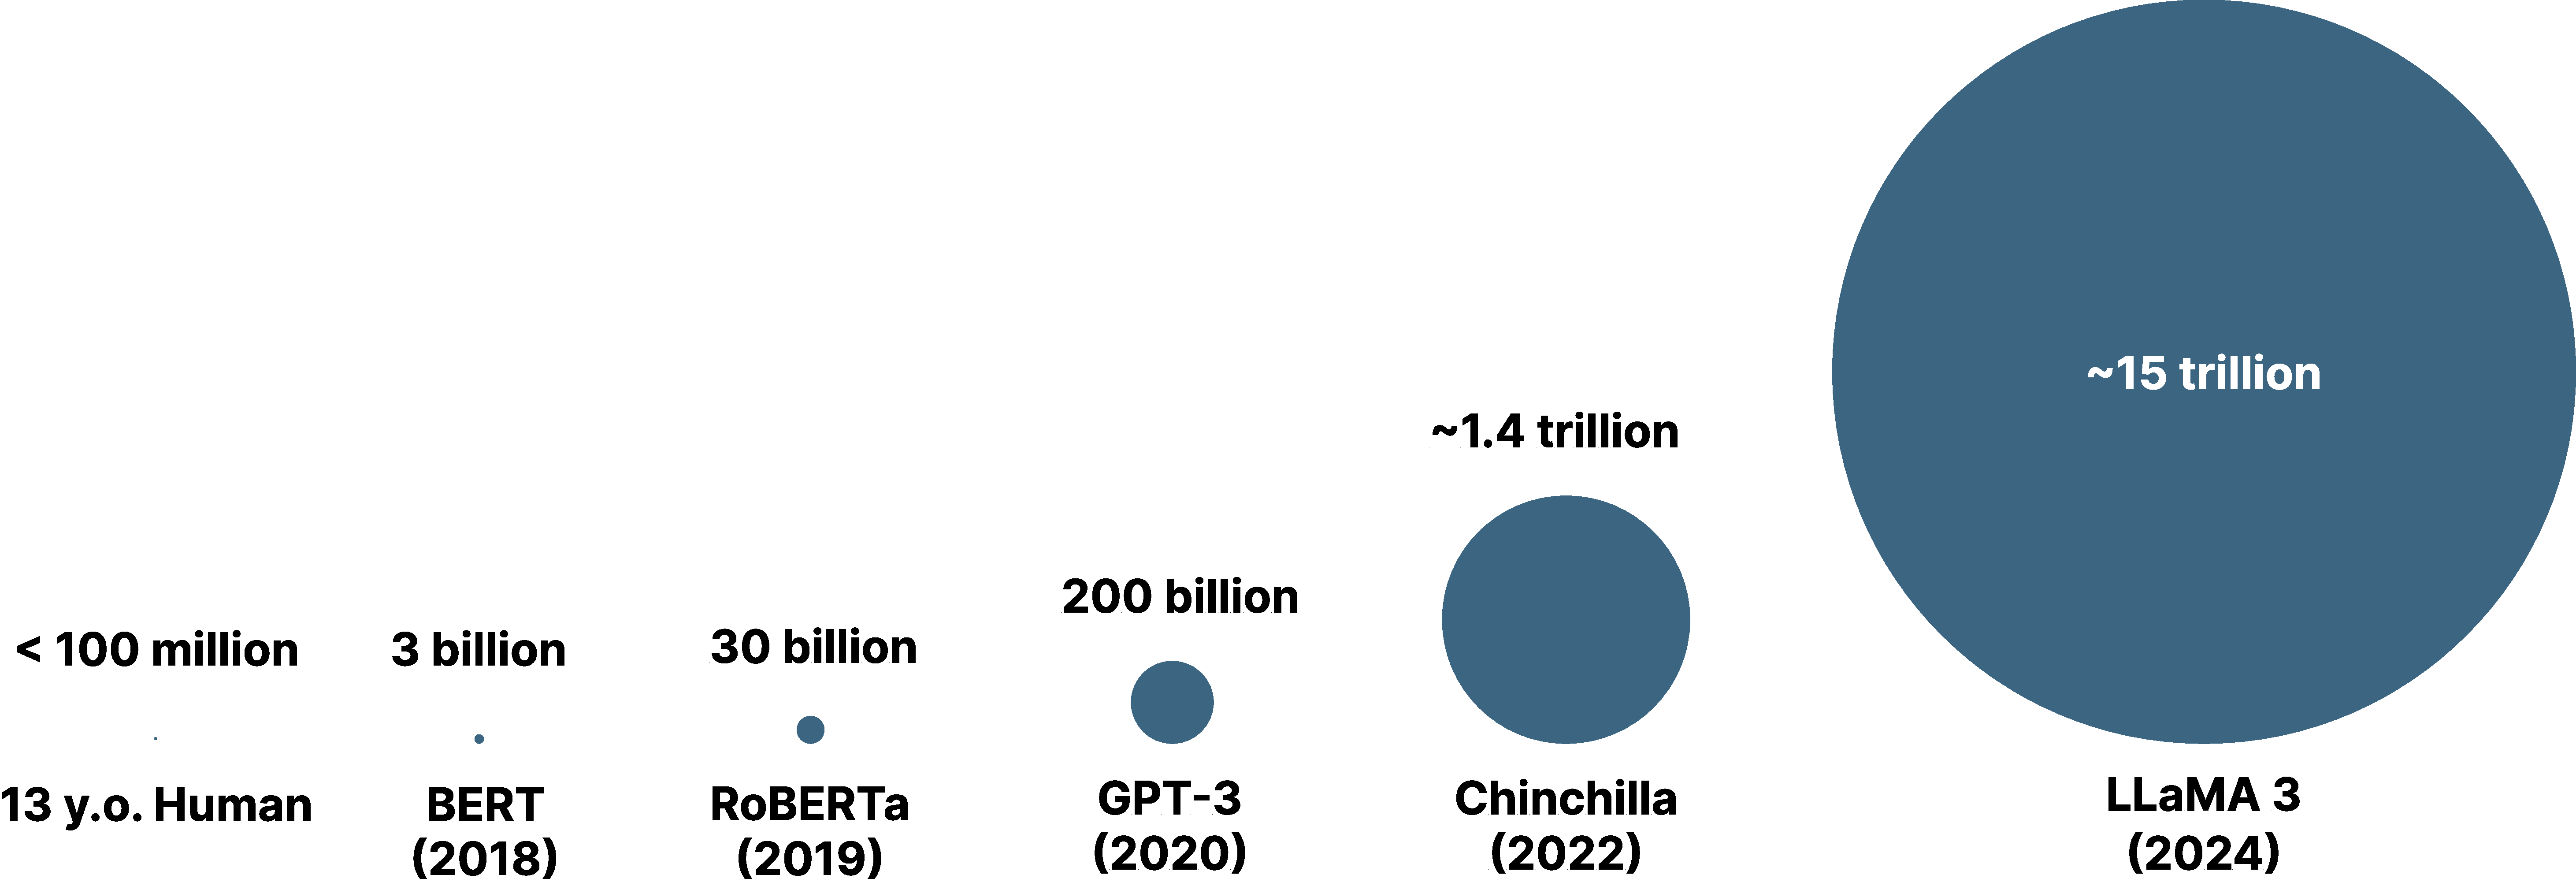
\includegraphics[width=0.7\textwidth]{chapters/background/figures/data_comparison.pdf}
    \caption{Comparison of data scales for different language modeling approaches.}
    \label{fig:data-comparison}
\end{figure}

The success of data calibration approaches and challenges like BabyLM raises an important question: where should we look for inspiration when developing more efficient and interpretable language models? While previous approaches have largely focused on architectural modifications to improve efficiency—such as reducing the quadratic complexity of attention mechanisms or optimizing memory bandwidth through innovations like flash attention—these solutions often emerge from engineering intuition rather than principled understanding.

One promising direction is to examine how the human brain processes and learns language. The brain has evolved to be remarkably efficient at language processing, operating under severe biological constraints while maintaining impressive capabilities. By studying cognitive processes like attention, memory, and learning in humans, we can potentially derive interpretable strategies that inform the development of better language modeling tools. This cognitive perspective is particularly relevant for small language models, where efficiency and interpretability are crucial.

A key area where cognitive insights can inform model development is in data augmentation strategies. Rather than focusing solely on architectural modifications, we can look to how humans learn language through diverse experiences and exposure to varied linguistic patterns. The brain's ability to generalize from limited data and adapt to new contexts suggests that carefully designed data augmentation techniques could help small language models achieve better performance without increasing model size or complexity.

This cognitive approach to data augmentation represents a shift from purely engineering-driven solutions to strategies grounded in our understanding of human language learning. By drawing parallels between human cognitive processes and machine learning approaches, we can develop more interpretable and efficient methods for training small language models.

Research in human language acquisition reveals that optimal learning occurs when input complexity is carefully calibrated. The "Goldilocks Effect" \cite{kidd2012goldilocks} demonstrates that infants naturally seek out information that is neither too simple nor too complex, but rather at an optimal level of difficulty that maximizes learning. This principle has profound implications for how we might structure training data for language models. Rather than exposing models to random or uniformly complex inputs, we could design curricula that gradually increase in complexity, mirroring how children naturally progress from simple to more complex linguistic structures \cite{clark2015first}.

The quality and nature of linguistic input is also crucial. Studies of early language development show that children benefit from rich, contextualized language input \cite{bergelson2015early, weizman2001lexical}. This suggests that language models might learn more effectively from carefully curated, contextually rich examples rather than from massive but potentially noisy datasets. Furthermore, the brain's predictive processing of language \cite{caucheteux2023evidence} indicates that learning is most effective when there's a balance between predictable patterns and novel information, allowing for both pattern recognition and adaptation to new contexts.

These cognitive insights suggest that data augmentation strategies for language models could be enhanced by incorporating principles of optimal input complexity, contextual richness, and predictive processing. By aligning our training approaches with how humans naturally learn language, we may be able to develop more efficient learning protocols that require less data and computational resources while maintaining or improving model performance. This approach not only draws inspiration from cognitive science but also provides a theoretical foundation for why certain training strategies might be more effective than others.


\subsection{Curriculum Learning}

Building on these cognitive insights, curriculum learning \cite{bengio2009curriculum} provides a formal machine learning framework for implementing progressive learning strategies inspired by human development. The core idea is to optimize model performance by gradually increasing training difficulty over time according to a predefined schedule, mirroring how humans naturally progress from simpler to more complex concepts. This approach has shown promise in various domains, but its application to language modeling remains relatively unexplored, particularly in the context of small-scale training regimes.

The challenge of training language models with limited data has become increasingly important as the field grapples with the sustainability of large-scale training. While children acquire language skills from an estimated two to seven million words per year \cite{gilkerson2017mapping}, current language models require disproportionately larger training corpora to achieve similar generalization capabilities \cite{zhang2021need}. For instance, state-of-the-art models like Chinchilla are trained on 1.4 trillion words \cite{hoffman2022chinchilla}, making such training regimes economically and ecologically unsustainable \cite{izsak2021train}.

Recent work has explored various approaches to improve data efficiency in language modeling, including using smaller, well-curated corpora \cite{samuel2023ltgbert, gao2020pile} and careful hyperparameter selection \cite{geiping2023cramming}. However, these approaches primarily offer engineering solutions rather than cognitively-inspired frameworks for training language models from scratch. The conventional pre-training paradigm remains far removed from human language learning: models operate on a predetermined static vocabulary and optimize a monotonous training objective on randomly shuffled data.

Curriculum learning offers a promising direction for addressing this gap between human language acquisition and current language modeling approaches. Recent work has explored different aspects of curriculum learning in language modeling, including:

1. \textbf{Vocabulary-based approaches}: Some studies have investigated how to gradually introduce vocabulary items during training, though this has primarily focused on domain-specific applications \cite{soviany2022curriculum}. This aligns with psycholinguistic research showing how children's lexicons grow from a small set of words to a full vocabulary \cite{bergelson2015early, weizman2001lexical}.

2. \textbf{Data ordering strategies}: Research has explored both static difficulty assessment based on linguistic criteria \cite{campos2021curriculum, kocmi2017curriculum, liu2018curriculum, platanios2019competence} and dynamic assessment based on model behavior \cite{sachan2016easy, lalor2020dynamic}. These approaches implement the "Goldilocks effect" \cite{kidd2012goldilocks}, where learning is optimized when difficulty is neither too easy nor too hard.

3. \textbf{Objective function variation}: Some work has investigated simplifying the learning objective during early training stages, such as mapping rare words to hypernyms \cite{bai2022better} or using part-of-speech tags instead of full vocabulary items \cite{wang2023language, cui2022lert}. This reflects how children progress from basic linguistic categories to more complex language understanding \cite{alishahi2010computational, gleitman1990structural}.

These approaches demonstrate the potential of curriculum learning for developing more cognitively plausible and data-efficient language models. By aligning model training more closely with human language acquisition processes, we can potentially achieve better performance with limited data while gaining insights into the relationship between human and machine language learning. The challenge lies in systematically implementing and evaluating these curriculum learning strategies within a unified framework that can be applied to small-scale language modeling scenarios.

In the following chapter, we present our investigation of curriculum learning for language modeling within the context of the BabyLM Challenge. We implement and evaluate three distinct curriculum learning approaches - vocabulary curriculum, data curriculum, and objective curriculum - each inspired by different aspects of human language acquisition. Our work establishes a computational framework for categorizing and implementing curriculum learning strategies that simulate human language learning dynamics, while also providing insights into the effectiveness of these approaches for training small language models with limited data. Through this investigation, we aim to contribute both to the development of more efficient language models and to our understanding of how machine learning approaches can be informed by human language acquisition processes.
